\chapter{Detailed design}

In this chapter, every single class is described in terms of public interface
and functionality. Because of the fairly dynamic character of this project --
new ideas come and go -- this chapter will not be finished until the end of the
project and will probably change regularly.

\section{Files and directories}

All source code will be in the directory \texttt{src/}. All classes are in the
package \texttt{amber} or in a subpackage thereof. The Psyclone specification
file \texttt{psySpec.xml} is found in \texttt{data/}. External libraries that
are redistributed with \Amber\ are in \texttt{lib/}. The source of this
document, the traineeship report and the website are located in
\texttt{documentation/}.

The application is built using Apache
Ant\footnote{\url{http://ant.apache.org/}} and it can be imported into
Eclipse\footnote{\url{http://www.eclipse.org/}}. It requires Java SDK version
1.5 or greater.

\section{Classes}

\begin{figure}[htp]
  \centering
  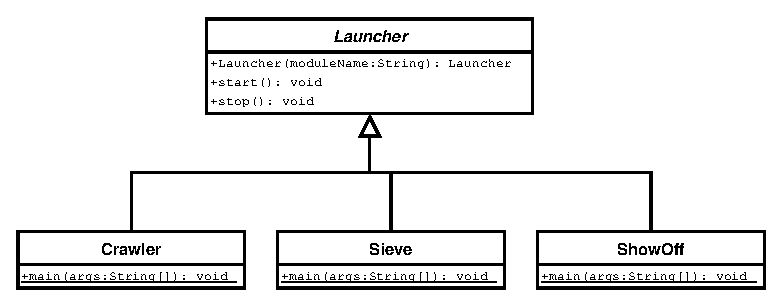
\includegraphics{image/class-diagram-launcher}
  \caption{The inheritance model of the Launcher class}
  \label{fig:class-diagram-launcher}
\end{figure}

\begin{figure}[p]
  \centering
  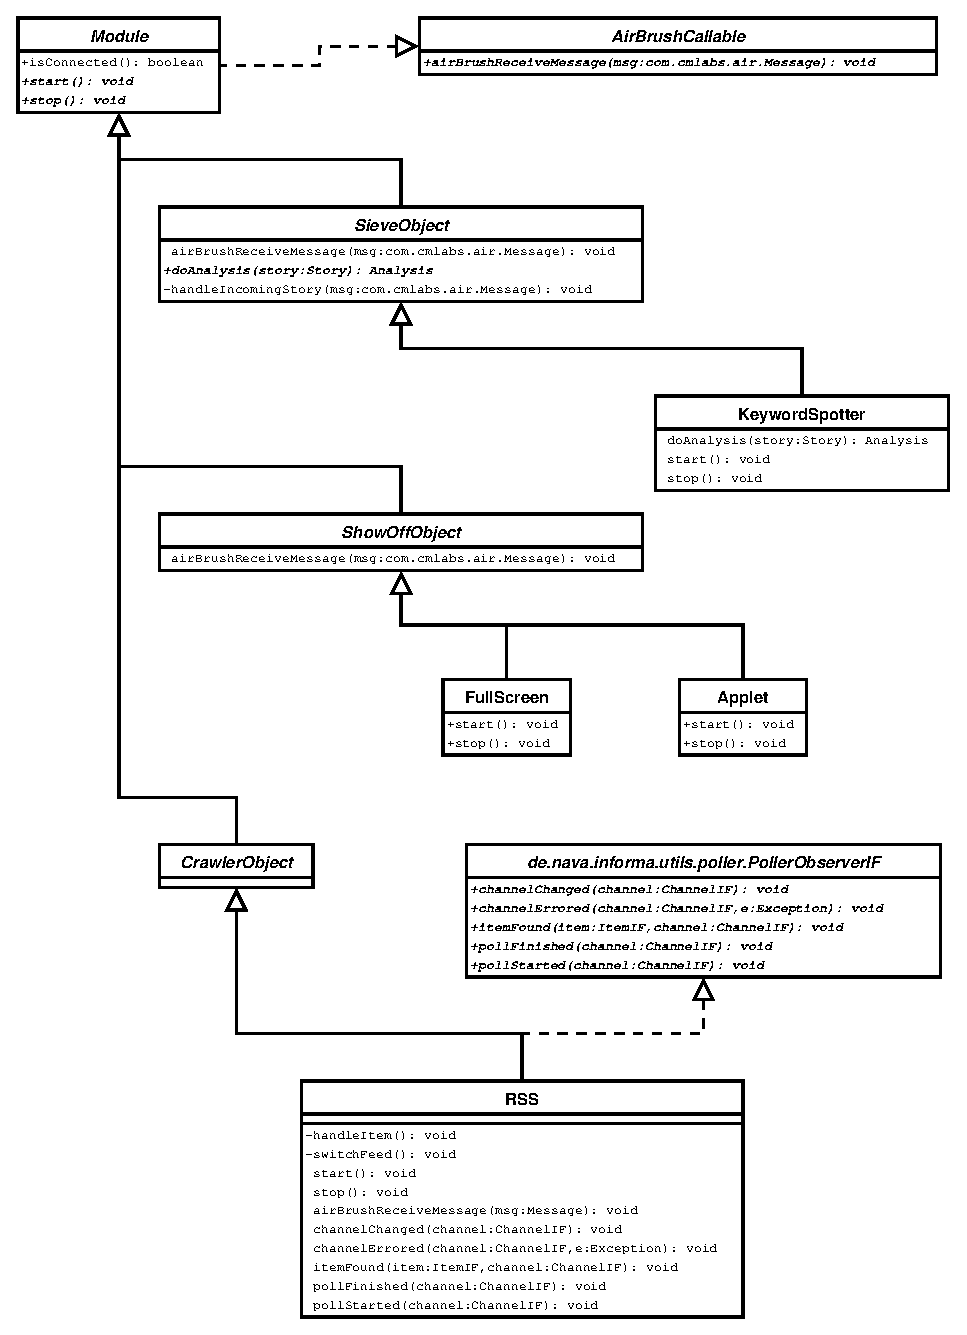
\includegraphics{image/class-diagram-module}
  \caption{The inheritance model of the Module class}
  \label{fig:class-diagram-launcher}
\end{figure}

\begin{figure}[p]
  \centering
  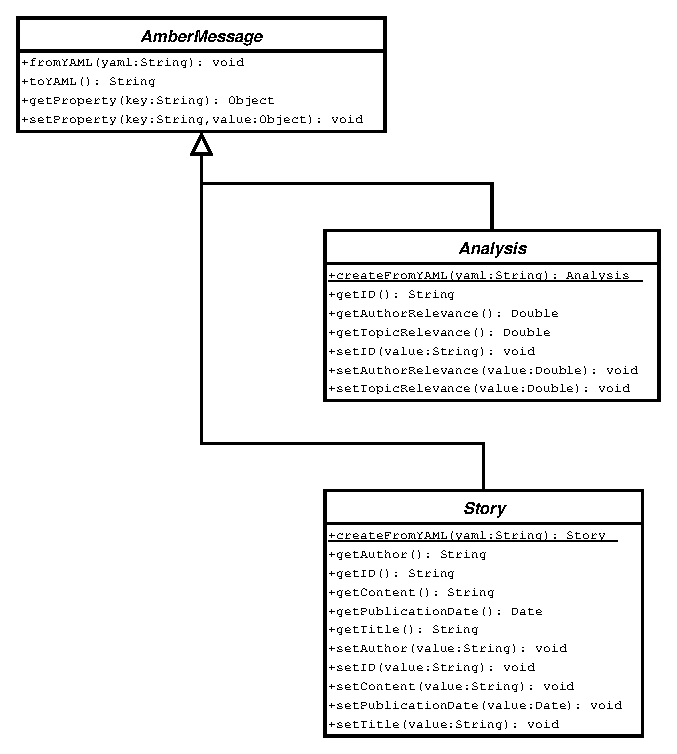
\includegraphics{image/class-diagram-ambermessage}
  \caption{The inheritance model of the AmberMessage class}
  \label{fig:class-diagram-launcher}
\end{figure}

\begin{figure}[p]
  \centering
  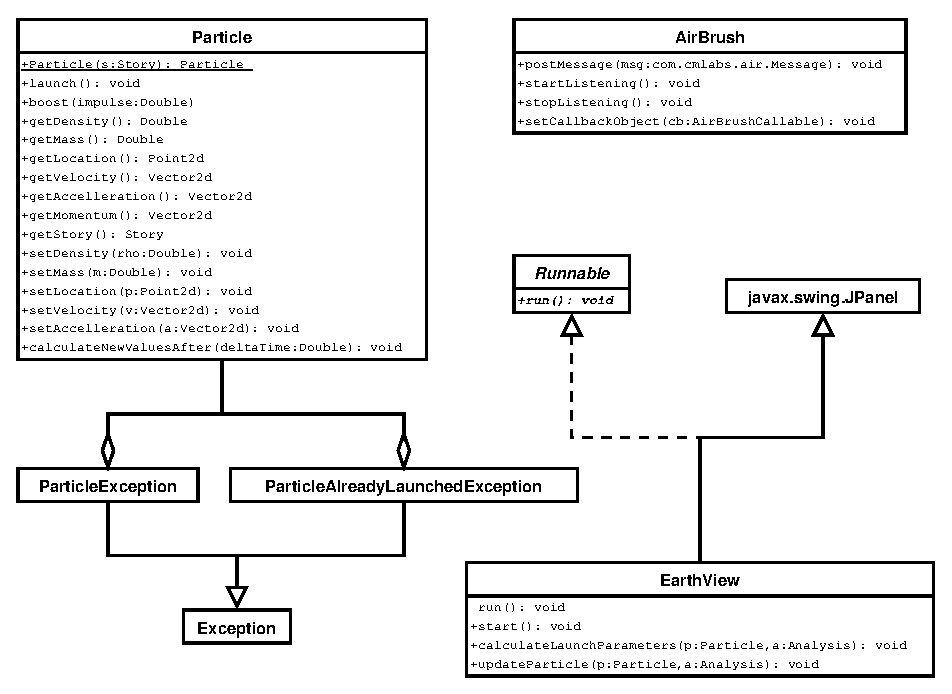
\includegraphics{image/class-diagram}
  \caption{The inheritance model of the remaining classes}
  \label{fig:class-diagram-launcher}
\end{figure}


\subsection{Objects in the amber package}

The classes in the main package are launchers for the three different modules
and abstract classes for the main objects of these modules. Basically it works
like this; if the Crawler class is started it creates a CrawlerObject and
starts it.

\classname{Crawler}

\begin{classmetadata}
  \function{The Crawler object makes launching a crawler easy and uniform for
      all crawler types.}
\end{classmetadata}

\begin{interface}
  \init{Crawler}{}
    {Creates an instance of Crawler. Also creates a CrawlerObject and the
      connection to Psyclone.}
  \method{\static\ \void}{main}{String\[\] args}
    {Method executed upon launch of the Crawler.}
  \method{\void}{start}{}
    {Starts the Crawler.}
  \method{\void}{stop}{}
    {Stops the Crawler.}
\end{interface}



\abstractclassname{CrawlerObject}

\begin{classmetadata}
  \function{The CrawlerObject class provides a uniform interface for crawler
      applications.}
  \implements{AirBrushCallable, ModuleInterface}
\end{classmetadata}



\classname{ShowOff}

\begin{classmetadata}
  \function{The ShowOff object makes launching a visualization module easy and
      uniform for all visualizer types.}
\end{classmetadata}

% \begin{interface}
% \end{interface}


\abstractclassname{ShowOffObject}

\begin{classmetadata}
  \function{The ShowOffObject class provides a uniform interface for visualization
      applications.}
  \implements{AirBrushCallable, ModuleInterface}
\end{classmetadata}

\begin{interface}
  \method{\void}{setStoryQueue}{\mbox{Queue$\langle$Story$\rangle$} q}
    {Sets the queue of incoming stories. ShowOff will handle communication with
      the Psyclone whiteboard and puts stories in the queue.}
\end{interface}



\classname{Sieve}

\begin{classmetadata}
  \function{The Sieve object makes launching a analysis module easy and uniform
      for all analyser types.}
\end{classmetadata}

% \begin{interface}
% \end{interface}



\abstractclassname{SieveObject}

\begin{classmetadata}
  \function{The SieveObject class provides a uniform interface for analysis
      applications.}
  \implements{AirBrushCallable, ModuleInterface}
\end{classmetadata}

% \begin{interface}
% \end{interface}



\section{Objects in the amber.common package}

\classname{AirBrush}

\begin{classmetadata}
  \function{Ease communication with Psyclone through JavaOpenAIR.}
\end{classmetadata}

\begin{interface}
  \init{AirBrush}{String moduleName, String hostName, int port}
    {Initializes a connection with Psyclone on \emph{hostName:port} for module
      \emph{moduleName}.}
  \method{\void}{setCallbackObject}{AirBrush\-Callable}
    {Sets the callback object to be used for calls from AirBrush.}
\end{interface}



\interfacename{AirBrushCallable}

\begin{interface}
  \method{\void}{airBrushCallBack}{com.cmlabs.air.Message msg}
    {Used as callback function for the AirBrush.}
\end{interface}



\interfacename{ModuleInterface}

\begin{interface}
  \method{\void}{start}{}
    {Start the module.}
  \method{\void}{stop}{}
    {Stop the module.}
\end{interface}



\classname{Story}

\begin{classmetadata}
  \function{Storage of Story data.}
  \data{Story has a Map$\langle$String, Object$\rangle$ field where it stores
    all data. It also holds a value with the number of analyses left until it
    is considered enough to be visualized. Instead of thrown back on the
    whiteboard with raw stories, it should then go the the processed stories.}
\end{classmetadata}

\begin{interface}
  \method{\static\ \void}{createFromYAML}{String yaml}
    {Creates a Story object, and initializes it from the \emph{yaml} argument
      (see fromYAML method).}
  \method{\void}{setAuthor}{String author}{Sets the author of the story.}
  \method{String}{getAuthor}{}{Gets the author of the story.}
  \method{\void}{setCreationTime}{Date time}{Set the creation time of the story}
  \method{Date}{getCreationTime}{}{Get the creation time of the story.}
  \method{\void}{setContent}{String text}{Set the content of the story.}
  \method{String}{getContent}{}{Get the content of the story.}
  \method{\void}{setValue}{String k, Object v}
    {Store an arbitrary object v under keyword k.}
  \method{Object}{getValue}{String k}
    {Gets the object stored under keyword k.}
  \method{Boolean}{lockForAnalysis}{}
    {Request a lock on the story for analysis. Returns true when given, assumes
      niceness of the analysis modules.}
  \method{\void}{unlock}{}
    {Removes the lock. Again, assumes niceness of the analysis modules.}
  \method{Boolean}{isAnalysisDone}{}
    {Returns true when the story finds it is analysed enough and doesn't need
      another run.}
  \method{\void}{fromYAML}{String yaml}
    {Parses a \ac{YAML} string (e.g. coming from Psyclone) to the contents of the
      object (overwrites values currently stored!). Note, together with toYAML,
      this is the identity function: story.fromYAML(story.toYAML()) = story.}
  \method{String}{toYAML}{}
    {Converts the contents of the object to a \ac{YAML} string to be sent via
      Psyclone.}
\end{interface}



\section{Objects in the amber.crawler package}



\classname{RSS}

\begin{classmetadata}
  \extends{CrawlerObject}
  \implements{AirBrushCallable}
  \processing{An RSS object will accept messages to set its feed source, i.e.
      the feed it should crawl. A message of type `Feed.RSS' or `Feed.Atom'
      will set the source to that URL, whereas a message of type `Feed.OMPL'
      will result RSS to parse this and set all URLs in the \ac{OPML} document
      as source URL.

      It will only post messages of the type `Story' as they are described in
      Section~\ref{sct:messages:story}. No other messages are sent.}
\end{classmetadata}

\begin{interface}
  \init{RSS}{}
    {Creates a new RSS crawler. It will wait for instructions via Psyclone,
      like which RSS feed has to be monitored.}
  \init{RSS}{URL feedurl}
    {Creates a new RSS crawler, initialized with the URL of the feed to be
      monitored.}
  \method{void}{airBrushReceiveMessage}{Message msg}
    {Callback function for AirBrushCallable. It will handle incoming messages
        of the type `Feed.RSS', `Feed.Atom' and `Feed.OPML'. With the OPML type
        it is possible to let a crawler handle more than one feed.}
  \method{void}{run}{}
    {Callback function for Runnable.}
\end{interface}

\begin{figure}
  \centering
  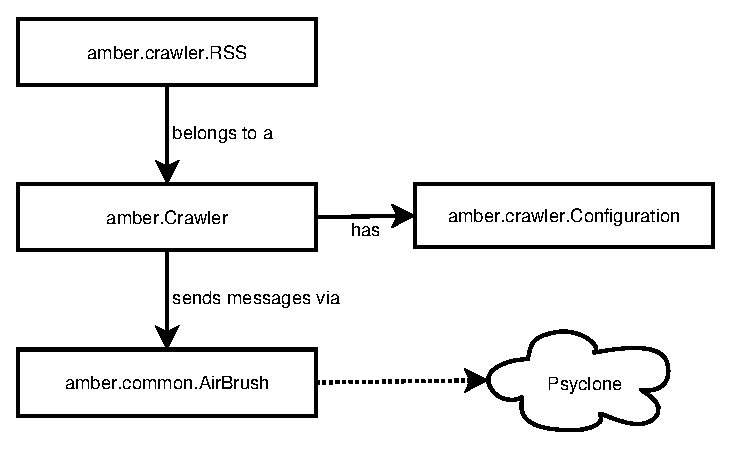
\includegraphics{image/crawler}
  \caption{
    Diagram of the design of the Crawler, the names are Java classnames, arrows
    mean that calls exist in the direction of the arrow.
  }
\end{figure}



\section{Objects in the amber.sieve package}

\classname{Configuration}

\begin{classmetadata}
\end{classmetadata}

\begin{interface}
\end{interface}



\classname{KeywordSpotter}

\begin{classmetadata}
  \implements{amber.common.AirBrushCallable}
\end{classmetadata}

\begin{interface}
\end{interface}



\section{Objects in the amber.showoff package}

\classname{Configuration}

\begin{classmetadata}
  \extends{amber.common.Configuration}
  \function{Store configuration}
\end{classmetadata}

\begin{interface}
  \method{void}{setValue}{String key}
    {Sets the value of key in the configuration.}
\end{interface}



\classname{EarthView}

\begin{classmetadata}
  \extends{java.awt.Canvas}
  \implements{Runnable}
\end{classmetadata}

\begin{interface}
  \init{EarthView}{}
    {Initializes the earthview display. It is a child of Canvas and can as such
    be used inside any application. Before starting the Earthview, first couple
    a Particle collection to it using setParticleCollection.}
  \method{\void}{setParticleCollection}{pc: Collection$\langle$Particle$\rangle$}
    {Sets the collection of particles to be displayed in the view.}
  \method{\void}{run}{}
    {Runs the thread (for Runnable).}
  \method{\void}{start}{}
    {Starts the thread, lets EarthView draw stuff.}
\end{interface}



\classname{FullScreen}

\begin{classmetadata}
  \extends{amber.ShowOffObject}
  \implements{amber.common.AirBrushCallable}
  % \function{}
\end{classmetadata}

\begin{interface}
  \init{FullScreen}{}
    {Initializes something.}
  \method{\void}{start}{}
    {Start the visualization.}
\end{interface}



\classname{Particle}

\begin{classmetadata}
  \function{Storage of particle data.}
  \data{An object of this class has information about its location and
    velocity, and it knows from which story it originates.}
\end{classmetadata}

\begin{interface}
  \init{Particle}{Story s}
    {Initializes a particle for Story s.}
  \method{\void}{launch}{}
    {Launches the particle, all parameters must be set, they cannot be changed
      afterwards.}
  \method{\void}{boost}{double}
    {Boost the particle in the direction it is heading. This can happen when
      for instance the Story gets replies or comments; boosting keeps the
      particle around longer.}
  \method{double}{getMass}{}
    {Gets the mass of the particle}
  \method{Vector$\langle$double$\rangle$}{getLocation}{}
    {Gets the location}
  \method{Vector$\langle$double$\rangle$}{getVelocity}{}
    {Gets the velocity}
  \method{Vector$\langle$double$\rangle$}{getAcceleration}{}
    {Gets the acceleration}
  \method{\void}{setMass}{double s}
    {Sets the mass of the particle to s}
  \method{\void}{setLocation}{Vector$\langle$double$\rangle$ v}
    {Sets the location to v}
  \method{\void}{setVelocity}{Vector$\langle$double$\rangle$ v}
    {Sets the velocity to v}
  \method{\void}{setAcceleration}{Vector$\langle$double$\rangle$ v}
    {Sets the acceleration to v}
  \method{\void}{setNewValuesAfter}{double t}
    {Calculates and sets new values using the current values after a period of
      time t}
\end{interface}



\classname{Applet}

\begin{classmetadata}
  \extends{java.applet.Applet}
\end{classmetadata}

\begin{interface}
\end{interface}



\begin{figure}
  \centering
  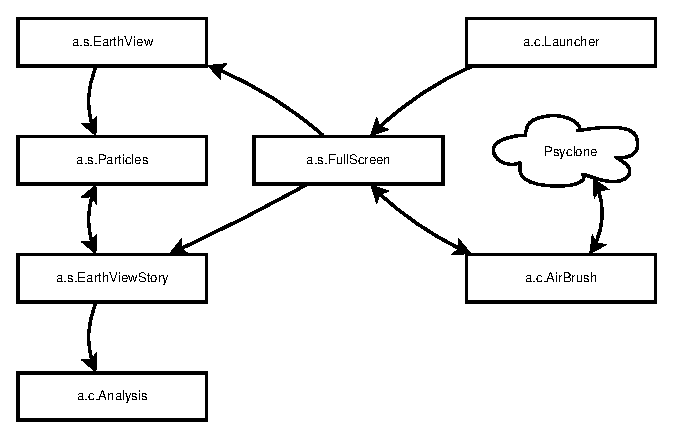
\includegraphics{image/showoff-fullscreen}
  \caption{
    Diagram of the design of the full screen ShowOff module, the names are
    abbreviated Java classnames
  }
\end{figure}



